% =====================================================================
%  CS375 Lab A11 - Simplified Filesystem with Security Features
%  Report
%
%  HOW TO USE
%   1. Edit your name / date in the "EDIT ME" block below.
%   2. Save screenshots into report/screenshots/ using EXACTLY the
%      file names listed in report/screenshots/README.md.
%      Missing screenshots show a grey placeholder box instead of failing.
%   3. Copy the numbers from your Test 9 screenshot into the \perf...
%      macros below so the performance table matches YOUR run.
%   4. Build:  make report   (from the project root)
% =====================================================================
\documentclass[11pt]{article}
\usepackage[margin=0.9in]{geometry}
\usepackage{amsmath}
\usepackage{graphicx}
\usepackage{float}
\usepackage{booktabs}
\usepackage{enumitem}
\usepackage{xcolor}
\usepackage{listings}
\usepackage{tikz}
\usetikzlibrary{positioning,arrows.meta}
\usepackage[hidelinks]{hyperref}

% ---------------------------- EDIT ME --------------------------------
\newcommand{\studentname}{Santiago Soto}
\newcommand{\course}{CS375 -- Operating Systems}
\newcommand{\labdate}{December 7, 2026}

% Performance numbers (copy from your ./fs_test 9 screenshot)
\newcommand{\perfFFSseqMs}{38.48}   \newcommand{\perfFFSseqNs}{1878.8}
\newcommand{\perfFFSrandMs}{39.96}  \newcommand{\perfFFSrandNs}{1951.4}
\newcommand{\perfFATseqMs}{32.23}   \newcommand{\perfFATseqNs}{1573.8}
\newcommand{\perfFATrandMs}{44.76}  \newcommand{\perfFATrandNs}{2185.8}
% ---------------------------------------------------------------------

% \screenshot{file name}{caption}  -> image, or a placeholder if missing
\newcommand{\screenshot}[2]{%
  \begin{figure}[H]
    \centering
    \IfFileExists{screenshots/#1}{%
      \includegraphics[width=\linewidth,height=0.80\textheight,keepaspectratio]{screenshots/#1}%
    }{%
      \fcolorbox{gray}{gray!10}{\parbox[c][3.2cm][c]{0.92\linewidth}{\centering
        \textbf{Screenshot not added yet}\\[4pt]
        save it as \texttt{report/screenshots/\detokenize{#1}}}}%
    }
    \caption{#2}
  \end{figure}}

\lstset{basicstyle=\ttfamily\small, columns=fixed, basewidth=0.5em, keepspaces=true, frame=single,
        breaklines=true, xleftmargin=4pt, xrightmargin=4pt}
\setlist{itemsep=2pt, topsep=3pt}

\title{\textbf{Lab A11: Designing and Implementing a Simplified\\
       Filesystem with Security Features}}
\author{\studentname \\ \course}
\date{\labdate}

\begin{document}
\maketitle

% =====================================================================
\section{Filesystem and Security Features}
% =====================================================================
I implemented \texttt{simplefs}, an in-memory simulation of an FFS-style
filesystem in C (\texttt{simplefs.c}, \texttt{simplefs.h}), plus a test
driver (\texttt{fs\_test.c}) that runs ten self-contained tests
(\texttt{./fs\_test 0}--\texttt{9}). The simulated disk is an array of
2048 blocks of 4\,KB, tracked by a free-block bitmap.

\paragraph{Filesystem features.}
\begin{itemize}
  \item \textbf{Inodes} hold size, a permission string (\texttt{rw-r-----}),
        owner UID, owning GID, reference count, timestamp, a group ACL,
        12 direct block pointers and one \textbf{single-indirect} pointer
        (Coding Task~1). The indirect block holds $4096/4 = 1024$ more
        pointers, so the maximum file size is $(12+1024)\times4\,\text{KB}
        \approx 4.05$\,MB.
  \item \textbf{First-fit block allocation} keeps a file's blocks next to
        each other, which mimics FFS block-group locality.
  \item \textbf{Directory} of name$\rightarrow$inode entries with
        \textbf{hard links} (shared inode, \texttt{ref\_count}++) and
        \textbf{soft links} (stored path, resolved at access time, with
        dangling-link and loop detection).
  \item \texttt{create}, \texttt{read}, \texttt{read\_at} (random access),
        \texttt{write} and \texttt{delete}. An inode and its blocks are
        freed only when \texttt{ref\_count} reaches 0, and freed blocks are
        zeroed.
\end{itemize}

\paragraph{Security features.}
\begin{itemize}
  \item \textbf{Access control:} owner $\rightarrow$ owning group
        $\rightarrow$ group ACL entries $\rightarrow$ other, checked on every
        read, write, link and delete. \textbf{Group-based ACLs}
        (Coding Task~2) give any group separate read and write rights. Only
        the owner may change a file's group or ACL.
  \item \textbf{Encryption at rest:} every data byte is XORed with key
        \texttt{0x55} before it is stored (it stands in for AES).
  \item \textbf{Secure log:} each operation, including \emph{denied} and
        \emph{failed} attempts, gets a sequence number and a keyed FNV-1a
        hash. The hash covers the text, timestamp, inode and the
        \emph{previous entry's hash}, which forms a hash chain.
        \texttt{verify\_logs()} recomputes every hash (Coding Task~3), and
        \texttt{print\_logs()} flags \texttt{[TAMPERED]} entries.
  \item \textbf{DoS limits:} a per-UID inode quota (64), a maximum file
        size and a symlink depth limit (8).
\end{itemize}

% =====================================================================
\section{Performance Analysis}
% =====================================================================
Test~9 reads a 1024-block (4\,MB) file 20 times, once in sequential block
order and once in a shuffled (random) order, which is 20{,}480 reads of
4\,KB per row. It also compares against a simulated \textbf{FAT} layout,
where the same blocks are scattered and linked through a
\texttt{next[]} table. Both layouts decrypt every byte, so the comparison
is fair.

\begin{table}[H]
\centering
\begin{tabular}{llrrr}
\toprule
Layout & Access & Total (ms) & Avg / block (ns) & Pointer lookups \\
\midrule
FFS (inode)      & Sequential & \perfFFSseqMs  & \perfFFSseqNs  & 40{,}720 \\
FFS (inode)      & Random     & \perfFFSrandMs & \perfFFSrandNs & 40{,}720 \\
FAT (linked list)& Sequential & \perfFATseqMs  & \perfFATseqNs  & 20{,}480 \\
FAT (linked list)& Random     & \perfFATrandMs & \perfFATrandNs & 10{,}496{,}000 \\
\bottomrule
\end{tabular}
\caption{Sequential vs.\ random access (see Figure~\ref{fig:perf}).}
\end{table}

\textbf{Analysis.} FFS random access (39.96\,ms) costs almost the same as
FFS sequential access (38.48\,ms, about 4\% faster), because the inode finds
any block in at most two lookups (direct pointer, or indirect block then
data block). FAT sequential access is the fastest row (32.23\,ms), because
it follows one link per block. Each FFS read also does a name lookup and a
permission check, and that per-call overhead accounts for most of the gap
to FAT sequential. FAT random access is the slowest row (44.76\,ms,
1.4$\times$ slower than FAT sequential): it must walk the chain from the
first cluster, which averages 512 hops per read, or 258$\times$ more
pointer lookups than FFS. In RAM a hop costs only nanoseconds, so most of
the time goes to decryption. On a real HDD each hop could be a separate
disk seek, so the FAT gap would be several orders of magnitude larger. FFS
block groups would also make sequential reads cheaper than random ones. Our
simulation does not model seeks, so that difference does not show up
here.

% =====================================================================
\section{Challenges Faced and Solutions}
% =====================================================================
\begin{enumerate}
  \item \textbf{Provided \texttt{fs\_test.c} did not compile.} It declared
        \texttt{extern struct simplefs} using incomplete types. I moved
        all structures and prototypes into a shared header,
        \texttt{simplefs.h}.
  \item \textbf{Stack overflow.} \texttt{struct simplefs} is over 8\,MB,
        so declaring it as a local variable in \texttt{main()} can crash.
        \texttt{fs\_create()} allocates it on the heap instead.
  \item \textbf{Wrong permission indices.} The original \texttt{read\_file}
        tested \texttt{permissions[4]} (the \emph{group-write} bit) to
        decide \emph{read} access, and \texttt{create\_hard\_link} tested
        \texttt{permissions[7]}. I rewrote the check to use owner [0--2],
        group [3--5] and other [6--8] correctly. To keep the expected
        output ``Permission denied for UID 1002'', the demo file uses
        \texttt{rw-r-----}.
  \item \textbf{Soft links read the wrong file.} The original soft-link
        entry kept \texttt{inode\_id = 0} from \texttt{memset}, so it only
        ``worked'' by accident. I added path resolution with dangling and
        loop detection.
  \item \textbf{Buffer overflow.} \texttt{buffer[inode->size] = '\textbackslash0'}
        wrote past \texttt{max\_len}. Reads are now limited to
        \texttt{max\_len - 1} bytes.
  \item \textbf{Weak log hash.} \texttt{id \^{} timestamp} can be
        recomputed by anyone. I replaced it with a keyed, chained hash, so
        editing, back-dating or forging an entry is detected.
\end{enumerate}

% =====================================================================
\section{Program Output (Screenshots)}
% =====================================================================
\screenshot{01_build.png}{Compiling with \texttt{make} (no warnings with
            \texttt{-Wall -Wextra}).}
\screenshot{02_test0_original_demo.png}{Test 0 -- the original lab driver:
            file creation, read, permission denied, hard and soft link
            reads, and the log.}
\screenshot{03_test1_basic.png}{Test 1 -- file creation and reading,
            directory listing and inode contents.}
\screenshot{04_test2_access_control.png}{Test 2 -- owner/group/other access
            control. Denied attempts are recorded in the log.}
\screenshot{05_test3_hard_links.png}{Test 3 -- hard links share one inode.
            Data survives until \texttt{ref\_count} reaches 0.}
\screenshot{06_test4_soft_links.png}{Test 4 -- soft links, dangling soft
            links after deletion, and loop detection.}
\screenshot{07_test5_indirect_blocks.png}{Test 5 -- Coding Task 1: a
            21-block file uses 12 direct pointers plus an indirect block.}
\screenshot{08_test6_encryption.png}{Test 6 -- the on-disk block holds
            ciphertext. An authorized read returns plaintext.}
\screenshot{09_test7_group_acls.png}{Test 7 -- Coding Task 2: group
            permission bits and group-based ACLs.}
\screenshot{10_test8_log_verification.png}{Test 8 -- Coding Task 3: log
            verification flags tampered entries.}
\screenshot{11_test9_performance.png}{Test 9 -- sequential vs.\ random
            access, FFS vs.\ FAT.\label{fig:perf}}

% =====================================================================
\section{Short-Answer Questions}
% =====================================================================
\begin{enumerate}[leftmargin=*]
\item \textbf{Inodes.} An inode stores a file's metadata: size, permissions,
  owner/group, timestamps, link (reference) count, and the direct, indirect
  and doubly-indirect pointers to its data blocks. It does not store the
  file name. Every operation goes through the inode: permission checks,
  finding data blocks for reads and writes, and deciding when a file can be
  freed. Without it the filesystem could neither find nor protect the data.

\item \textbf{Hard vs.\ soft links.} A hard link is another directory entry
  that points to the \emph{same inode}. A soft link is a separate entry
  that stores a \emph{path name} and is resolved each time it is used.
  Because several names share one inode, the filesystem needs a reference
  count to know when the last name is gone. Only then can it free the inode
  and its blocks; otherwise it would free data that is still reachable, or
  leak it forever.

\item \textbf{Block groups.} FFS divides the disk into block groups, each
  with its own inodes, bitmaps and data blocks. It places a file's inode,
  its data and its directory in the same group. This keeps related data
  physically close, so the HDD head makes short seeks. FAT has one table at
  the start of the disk and allocates clusters anywhere, so a file can be
  scattered, and the head keeps travelling between the FAT and distant data.

\item \textbf{Access control.} Before every read, write, link or delete,
  \texttt{check\_permission()} compares the caller's UID with the inode's
  owner bits, then its group bits and group ACL entries, then its ``other''
  bits, and the operation is refused if the right bit is missing. Least
  privilege matters because each unneeded permission is extra attack
  surface. If an account or program is compromised, the damage is limited
  to what it really needed.

\item \textbf{Encryption.} Encryption keeps data confidential even if
  permissions are bypassed, for example when a disk is stolen, a raw block
  is read, or a backup leaks, because without the key the blocks are
  ciphertext. The trade-offs are CPU time for every read and write (which
  AES-NI hardware reduces), the work of managing keys (lost key means lost
  data), and less effective compression and deduplication.

\item \textbf{Secure logging.} Each entry's hash is computed over its
  contents, a secret key and the previous entry's hash.
  \texttt{verify\_logs()} recomputes it and compares it to the stored value.
  If someone edits an entry (for example, to hide a denied access), the
  recomputed hash no longer matches and the entry is flagged
  \texttt{[TAMPERED]}. If someone deletes, reorders or re-hashes an entry,
  the chain to the following entry breaks, which is detected as well.
\end{enumerate}

% =====================================================================
\section{Long-Answer Questions}
% =====================================================================
\subsection{Inode-Based Filesystems (FFS vs.\ FAT)}
In FFS every file has one inode in a fixed inode table. A directory maps a
name to an inode number. The inode holds metadata and a tree of block
pointers: 12 direct pointers, then single-, double- and triple-indirect
blocks. To read byte $b$ the OS computes the logical block $k=\lfloor
b/4096\rfloor$. If $k<12$ it uses \texttt{direct[k]}; otherwise it reads the
indirect block and indexes it at $k-12$. Locating any block therefore takes
a constant, small number of lookups (at most 4), however large the file is.

FAT stores a file as a linked list: the directory gives the first cluster,
and \texttt{FAT[c]} gives the next one. Sequential reads are cheap (one hop
per block), so FAT and FFS are comparable there, although FFS block groups
lay data out more contiguously. Random access is where FFS wins. Reaching
block $k$ in FAT requires following $k$ links, which is $O(n)$, while FFS
indexes the pointer tree directly, which is $O(1)$. My Test~9 confirms
this: FAT needed 10.5 million pointer hops for random reads, while FFS
needed 40{,}720.

\begin{center}
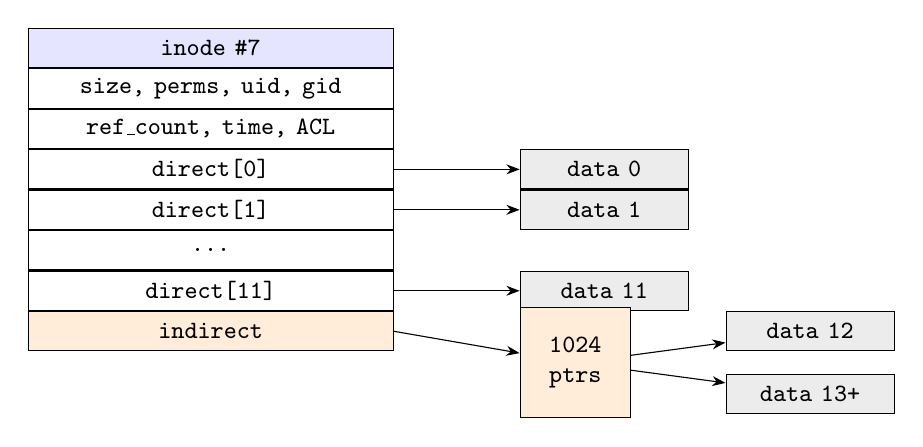
\begin{tikzpicture}[font=\small\ttfamily, node distance=2mm,
  box/.style={draw, text width=4.4cm, align=center, minimum height=5mm, anchor=west},
  blk/.style={draw, fill=gray!15, text width=1.9cm, align=center, minimum height=5mm},
  ->, >=Stealth]
  \node[box, fill=blue!10] (h) {inode \#7};
  \node[box, below=0mm of h.south west, anchor=north west] (m1) {size, perms, uid, gid};
  \node[box, below=0mm of m1.south west, anchor=north west] (m2) {ref\_count, time, ACL};
  \node[box, below=0mm of m2.south west, anchor=north west] (d0) {direct[0]};
  \node[box, below=0mm of d0.south west, anchor=north west] (d1) {direct[1]};
  \node[box, below=0mm of d1.south west, anchor=north west] (dd) {\dots};
  \node[box, below=0mm of dd.south west, anchor=north west] (d11) {direct[11]};
  \node[box, below=0mm of d11.south west, anchor=north west, fill=orange!15] (ind) {indirect};
  \node[blk, right=1.6cm of d0] (b0) {data 0};
  \node[blk, right=1.6cm of d1] (b1) {data 1};
  \node[blk, right=1.6cm of d11] (b11) {data 11};
  \node[draw, fill=orange!15, minimum width=1.4cm, minimum height=1.4cm,
        right=1.6cm of ind, yshift=-4mm, align=center] (ib) {1024\\ptrs};
  \node[blk, right=1.2cm of ib, yshift=4mm] (b12) {data 12};
  \node[blk, right=1.2cm of ib, yshift=-4mm] (b13) {data 13+};
  \draw (d0.east) -- (b0); \draw (d1.east) -- (b1); \draw (d11.east) -- (b11);
  \draw (ind.east) -- (ib); \draw (ib) -- (b12); \draw (ib) -- (b13);
\end{tikzpicture}
\end{center}

\subsection{Hard and Soft Links}
\textbf{Implementation.} A \emph{hard link} is a new directory entry that
holds an \emph{existing inode number}, and the inode's \texttt{ref\_count}
is incremented. The two names are equal, and neither is the ``original''. A
\emph{soft link} is a directory entry whose data is a \emph{path string}.
On access, the filesystem looks that path up again and repeats the lookup
for chained links. It enforces a depth limit to stop loops (my code returns
\texttt{FS\_ERR\_LOOP} after 8 hops).

\textbf{Deletion and space.} Deleting a name only decrements
\texttt{ref\_count}. The inode and its blocks are freed when the count
reaches zero (Test~3). This means deleting a file does not always free
space: a forgotten hard link can keep a large file alive. A hard link costs
only a directory entry. A soft link costs an entry (in real systems also a
small inode) but never keeps its target alive. Hard links cannot cross
filesystems or point to directories, because inode numbers are only unique
within one filesystem and directory links could create cycles. Soft links
can do both.

\begin{lstlisting}
delete(name): e = lookup(name); remove e
  if !e.soft: inode.ref--; if inode.ref == 0: free(inode, blocks)
\end{lstlisting}

\textbf{Failing scenario.} \texttt{config -> /etc/app/config.v1}. An admin
renames the file to \texttt{config.v2}, or the disk holding the target is
unmounted. The soft link now points to a path that does not exist, so
reading it fails with ``No such file'' (Test~4: dangling link). A hard link
would still work.

\subsection{Access Control and Security}
Traditional Unix permissions allow exactly one owner, one group and
``everyone else''. If two teams need different rights to the same file,
the only option is to create a new group or to make the file
world-readable, which violates least privilege. \textbf{ACLs} attach a list
of (group or user, rights) entries to each inode, so the owner can grant
\emph{auditors} read-only access and \emph{developers} read-write access at
the same time (Test~7), without exposing the file to anyone else. They make
fine-grained least privilege practical and auditable.

\textbf{Vulnerability.} In the provided code, \texttt{read\_file} granted
read access if \texttt{permissions[4] == 'r'}, but index~4 is the
\emph{group-write} bit, and \texttt{create\_hard\_link} likewise tested
the wrong bit. A related escalation is letting a non-owner edit ACLs. An
attacker with UID 1004 calls \texttt{add\_acl\_entry(file, 1004, ...)} on
a file that is not theirs, grants their group \texttt{rw}, and then
reads or overwrites it. A third issue is creating a hard link to a
privileged file, so the attacker keeps access after the file is ``deleted''.

\textbf{Mitigation} (all implemented):
\begin{lstlisting}
check_permission(inode, uid, mode):
  if uid == owner:          return owner_bit(mode)
  if uid in inode.gid:      if group_bit(mode): return true
  for a in inode.acl:       if uid in a.gid and a.allows(mode): return true
  return other_bit(mode)    # unless uid matched owning group
add_acl_entry/set_file_group: require uid == owner, else log DENIED
hard link / delete:           require owner or write permission
\end{lstlisting}
Every denied attempt is logged, so escalation attempts are visible.

\subsection{Encryption and Logging}
\textbf{Encryption} converts each block to ciphertext with a key that is not
stored next to the data (Test~6 shows ciphertext on disk). An attacker who
bypasses the OS, for example by stealing the drive, reading raw blocks or
copying a backup, sees only ciphertext. Production systems use AES-XTS (as
in LUKS, BitLocker or fscrypt). The simple XOR here only demonstrates the
idea.

\textbf{Secure logging} records who did what and when, including denied
attempts. Repeated \texttt{DENIED read payroll.txt by UID 1002} entries
reveal unauthorized probing. A keyed, chained hash makes the trail itself
tamper-evident (Test~8), so an intruder cannot quietly erase their tracks.

\textbf{Trade-offs.}
\begin{itemize}
  \item \emph{Encrypt everything:} simple, with no risk of forgetting a
        sensitive file, and it covers temporary files, swap and metadata.
        The cost is CPU time on every I/O (small with AES-NI), plus losing
        the key loses the whole disk. Compression and deduplication also
        become harder.
  \item \emph{Selective encryption:} lower overhead and keys can be held
        per user or per directory, but it depends on users classifying data
        correctly, and plaintext copies can leak into unencrypted temp files
        or logs.
\end{itemize}

\textbf{Use case.} A hospital laptop holding patient records (HIPAA) should
use full-disk encryption, so a lost laptop is not a breach. The records
server should add per-directory encryption keys for each department and
tamper-evident access logs. Auditors can then prove who viewed which record.

\end{document}
